\documentclass[10pt,twocolumn,twoside]{genpaper}
\usepackage[numbers,sort&compress]{natbib}

\newcommand{\vg}{$\mathtt{vg}$}
\newcommand{\mg}{$\mathtt{minigraph}$}
\newcommand{\sw}{$\mathtt{seqwish}$}
\newcommand{\minimap}{$\mathtt{minimap2}$}
\newcommand{\miniasm}{$\mathtt{miniasm}$}
\newcommand{\bwa}{$\mathtt{BWA\text{-}MEM}$}

\newcommand{\ec}{\emph{E.~coli}}
\newcommand{\sce}{\emph{S.~cerevisae}}
\newcommand{\kp}{\emph{K.~pneumoniae}} 

\newcommand{\IE}{\emph{i.e.}}
\newcommand{\EG}{\emph{e.g.}}
\newcommand{\review}[1]{\textcolor{red}{#1}}

\newcommand{\cthead}[2]{\multicolumn{#1}{c}{\textbf{#2}}}
\definecolor{Gray}{gray}{0.9}
\newcommand{\cir}{$^\ast$}
\newcommand{\bres}[1]{{\bf #1}}

\usepackage{pdfpages} 
\usepackage{mathtools}
\usepackage{play}
\usepackage{makeidx}
\usepackage{xcolor,colortbl}
\usepackage{longtable}
\usepackage{booktabs}
\usepackage{hyperref}
\usepackage{pdflscape}

\usepackage{amsmath,amsfonts,amssymb} % this is handy for mathematicians and physicists
			      % see http://www.ams.org/tex/amslatex.html

% \usepackage{showkeys} % this shows what labels you are using for cross
		      % references

\usepackage{graphicx} % standard graphics package for inclusion of
		      % images and eps files into LaTeX document

\usepackage{multirow} 

\usepackage{float}
\usepackage[caption = false]{subfig}
% this code hacked from that of R Chandrasekhar from UWA
\newif\ifpdf
\ifx\pdfoutput\undefined
	\pdffalse    % we are not running pdfLaTeX
\else
	\pdfoutput=1 % we are running pdfLaTeX
	\pdftrue
\fi

\ifpdf
	\DeclareGraphicsExtensions{.pdf}  % this command defined in graphicx
	\pdfcompresslevel=9  % 0: no compression, 9: highest compression
			     % or, set compress_level 9 in file pdftex.cfg
\else
	\DeclareGraphicsExtensions{.ps}
\fi

%\usepackage{xr}
%\externaldocument{supplementary}
%%%%%%%%%%%%%%%%%%%%%%%%%%%%%%%%%%%%%%%%%%%%%%%%%%%%%%%%%%%%%%%%%%%%%%%%%%%%%%
%%%%%%%%%%%%%%%%%%%%%%%%%%%%%%%%%%%%%%%%%%%%%%%%%%%%%%%%%%%%%%%%%%%%%%%%%%%%%%
%% Some functions provided  by the class

%Display line numbers on the margins
\lineno

%Display watermark DRAFT
%\watermark{DRAFT}

%% use \onecolumn for onecolumn paper
\onecolumn

\title{Application of genome graph in AMR profiling}
\shorttitle{Genome graph}

%Authors
\author[1,$\ast$]{AMROMIC}

%Affiliation
\affil[1]{Vietnam-Australia-USA}
\correspondingauthor{
\textsuperscript{$\ast$}
To whom correspondence should be addressed. 
E-mails: aba@xyz.com
}

%Display ``This manuscript was compiled on XXXX''
\compiledate

%Set abstract (see below)
\abstract{Genome graph has been proposed and applied in genomics as the solution for a better reference system to increase mapping quality and variant calling performance. Even at early stage, this direction shows promising results in human genomics and metagenomics. In this study, we are forcus on the application of this technique to build a pangenome suitable for resistomes. The results are expected to presented more comprehensive insights into structural variants (SV) that are correlated to the resistance behaviour of the fast-growing superbugs.}
 
%Set keywords
\keywords{microbial genomics, pangenome, genome graph, antibiotic resistance}

%%%%%%%%%%%%%%%%%%%%%%%%%%%%%%%%%%%%%%%%%%%%%%%%%%%%%%%%%%%%%%%%%%%%%%%%%%%%%%

\begin{document}
%Abstract and keywords have to be defined before \maketitle
\maketitle
\thispagestyle{fancy}

%%%%%%%%%%%%%%%%%%%%%%%%%%%%%%%%%%%%%%%%%%%%%%%%%%%%%%%%%%%%%%%%%%%%%%%%%%%%%%%%%%%
\section*{Background}
The idea of pangenome graph had been proposed long ago as a proof-of-concept for a comprehensive but compact reference model. After having a genome graph, we can align a query sequence directly to the graph for variant calling. There were improvement in terms of mapping rate \vg{} tool sets (\url{https://github.com/vgteam/vg}) had been developed for this purpose and currently the most active project working on this field. 

\begin{figure}[!hpt]
\centering
\caption{Example of a genome graph, steal from \vg{}.}
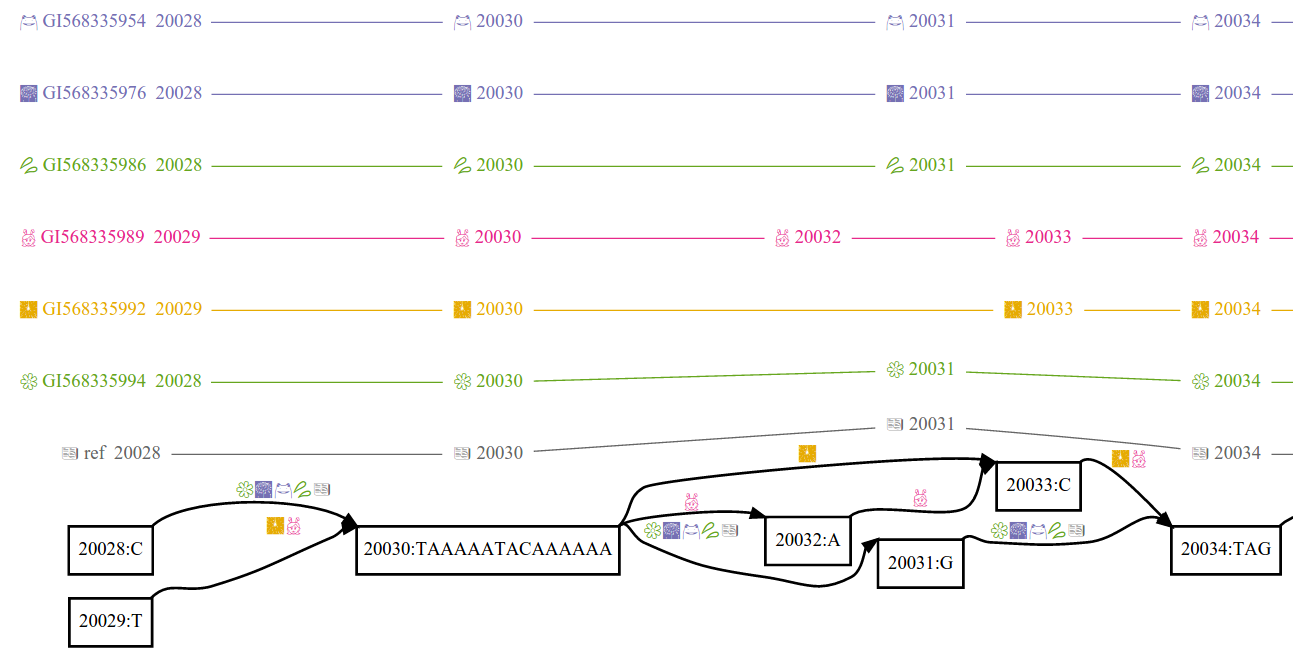
\includegraphics[width=.9\textwidth]{images/smallgraph.png}
\end{figure}

To date, there are two practical implementations for pangenome graph construction to considered:
\begin{itemize}
\item \url{https://github.com/lh3/minigraph}: \emph{reference model} that focus on a stable, linear cooridnate system of the reference genome thus restraint the graph structure. The graph can be build progressively.
\item \url{https://github.com/ekg/seqwish}: more flexible graph using a \emph{path model} that can incorporate multiple references, created by all-to-all pairwise alignment.
\end{itemize}

Resources to considered:
\begin{itemize}
\item Tools on github: \vg{}, \mg{}, \sw{}, $\mathtt{cactus}$
\item Sites: \url{https://www.sevenbridges.com/graph/}, \url{https://ekg.github.io/}, \url{https://lh3.github.io/}
\item Debate: \url{https://github.com/lh3/gfatools/issues/1}
\end{itemize}
\section*{Technical focus}
One way to construct the genome graph is to integrate a variant catalog (VCF file) into a reference. This is a common practice for human genome when we have a stable reference and a set of known variants output in a VCF file.

Another option is to build the graph on the assembly sequences from the beginning.
One problem addressed by researcher when constructing a genome graph progressively is the unavoidable \emph{reference bias}.
\sw{} try to avoid this by aligning all pairs of sequences together, sacrificing the ability to integrate genomes into the graph one-by-one from the very beginning.
\section*{Results}

\bibliographystyle{pnas2011}
\bibliography{library} 

\end{document}
